% GNUPLOT: LaTeX picture with Postscript
\begingroup
  \makeatletter
  \providecommand\color[2][]{%
    \GenericError{(gnuplot) \space\space\space\@spaces}{%
      Package color not loaded in conjunction with
      terminal option `colourtext'%
    }{See the gnuplot documentation for explanation.%
    }{Either use 'blacktext' in gnuplot or load the package
      color.sty in LaTeX.}%
    \renewcommand\color[2][]{}%
  }%
  \providecommand\includegraphics[2][]{%
    \GenericError{(gnuplot) \space\space\space\@spaces}{%
      Package graphicx or graphics not loaded%
    }{See the gnuplot documentation for explanation.%
    }{The gnuplot epslatex terminal needs graphicx.sty or graphics.sty.}%
    \renewcommand\includegraphics[2][]{}%
  }%
  \providecommand\rotatebox[2]{#2}%
  \@ifundefined{ifGPcolor}{%
    \newif\ifGPcolor
    \GPcolorfalse
  }{}%
  \@ifundefined{ifGPblacktext}{%
    \newif\ifGPblacktext
    \GPblacktexttrue
  }{}%
  % define a \g@addto@macro without @ in the name:
  \let\gplgaddtomacro\g@addto@macro
  % define empty templates for all commands taking text:
  \gdef\gplbacktext{}%
  \gdef\gplfronttext{}%
  \makeatother
  \ifGPblacktext
    % no textcolor at all
    \def\colorrgb#1{}%
    \def\colorgray#1{}%
  \else
    % gray or color?
    \ifGPcolor
      \def\colorrgb#1{\color[rgb]{#1}}%
      \def\colorgray#1{\color[gray]{#1}}%
      \expandafter\def\csname LTw\endcsname{\color{white}}%
      \expandafter\def\csname LTb\endcsname{\color{black}}%
      \expandafter\def\csname LTa\endcsname{\color{black}}%
      \expandafter\def\csname LT0\endcsname{\color[rgb]{1,0,0}}%
      \expandafter\def\csname LT1\endcsname{\color[rgb]{0,1,0}}%
      \expandafter\def\csname LT2\endcsname{\color[rgb]{0,0,1}}%
      \expandafter\def\csname LT3\endcsname{\color[rgb]{1,0,1}}%
      \expandafter\def\csname LT4\endcsname{\color[rgb]{0,1,1}}%
      \expandafter\def\csname LT5\endcsname{\color[rgb]{1,1,0}}%
      \expandafter\def\csname LT6\endcsname{\color[rgb]{0,0,0}}%
      \expandafter\def\csname LT7\endcsname{\color[rgb]{1,0.3,0}}%
      \expandafter\def\csname LT8\endcsname{\color[rgb]{0.5,0.5,0.5}}%
    \else
      % gray
      \def\colorrgb#1{\color{black}}%
      \def\colorgray#1{\color[gray]{#1}}%
      \expandafter\def\csname LTw\endcsname{\color{white}}%
      \expandafter\def\csname LTb\endcsname{\color{black}}%
      \expandafter\def\csname LTa\endcsname{\color{black}}%
      \expandafter\def\csname LT0\endcsname{\color{black}}%
      \expandafter\def\csname LT1\endcsname{\color{black}}%
      \expandafter\def\csname LT2\endcsname{\color{black}}%
      \expandafter\def\csname LT3\endcsname{\color{black}}%
      \expandafter\def\csname LT4\endcsname{\color{black}}%
      \expandafter\def\csname LT5\endcsname{\color{black}}%
      \expandafter\def\csname LT6\endcsname{\color{black}}%
      \expandafter\def\csname LT7\endcsname{\color{black}}%
      \expandafter\def\csname LT8\endcsname{\color{black}}%
    \fi
  \fi
    \setlength{\unitlength}{0.0500bp}%
    \ifx\gptboxheight\undefined%
      \newlength{\gptboxheight}%
      \newlength{\gptboxwidth}%
      \newsavebox{\gptboxtext}%
    \fi%
    \setlength{\fboxrule}{0.5pt}%
    \setlength{\fboxsep}{1pt}%
\begin{picture}(7200.00,5040.00)%
    \gplgaddtomacro\gplbacktext{%
      \csname LTb\endcsname%
      \put(3600,4453){\makebox(0,0){\strut{}}}%
      \put(220,220){\makebox(0,0)[l]{\strut{}}}%
    }%
    \gplgaddtomacro\gplfronttext{%
      \csname LTb\endcsname%
      \put(3529,3950){\makebox(0,0){\strut{}}}%
      \csname LTb\endcsname%
      \put(5400,3950){\makebox(0,0)[r]{\strut{}T=0 single pair excitation region}}%
      \csname LTb\endcsname%
      \put(5400,3730){\makebox(0,0)[r]{\strut{}Zeros of Re($\varepsilon$)}}%
      %Draw the cyan line by hand
      \put(5500,3730){\makebox(0,0)[l]{\strut{}\textcolor{cyan}{\rule[3pt]{28pt}{1pt}}}}%
      \csname LTb\endcsname%
      \put(5400,3510){\makebox(0,0)[r]{\strut{}$\omega_{TO}$}}%
      \csname LTb\endcsname%
      \put(936,604){\makebox(0,0){\strut{} 0}}%
      \put(1469,604){\makebox(0,0){\strut{} 0.5}}%
      \put(2002,604){\makebox(0,0){\strut{} 1}}%
      \put(2535,604){\makebox(0,0){\strut{} 1.5}}%
      \put(3068,604){\makebox(0,0){\strut{} 2}}%
      \put(3600,604){\makebox(0,0){\strut{} 2.5}}%
      \put(4132,604){\makebox(0,0){\strut{} 3}}%
      \put(4665,604){\makebox(0,0){\strut{} 3.5}}%
      \put(5198,604){\makebox(0,0){\strut{} 4}}%
      \put(5731,604){\makebox(0,0){\strut{} 4.5}}%
      \put(6264,604){\makebox(0,0){\strut{} 5}}%
      \csname LTb\endcsname%
      \put(3600,274){\makebox(0,0){\strut{}Wave vector $k/k_F$}}%
      \csname LTb\endcsname%
      \put(748,917){\makebox(0,0)[r]{\strut{} 0}}%
      \put(748,1452){\makebox(0,0)[r]{\strut{} 1}}%
      \put(748,1986){\makebox(0,0)[r]{\strut{} 2}}%
      \put(748,2520){\makebox(0,0)[r]{\strut{} 3}}%
      \put(748,3054){\makebox(0,0)[r]{\strut{} 4}}%
      \put(748,3588){\makebox(0,0)[r]{\strut{} 5}}%
      \put(748,4123){\makebox(0,0)[r]{\strut{} 6}}%
      \csname LTb\endcsname%
      \put(418,2520){\rotatebox{-270}{\makebox(0,0){\strut{}Energy $E/E_F$}}}%
      \csname LTb\endcsname%
      \put(6796,917){\makebox(0,0)[l]{\strut{} 0}}%
      \put(6796,1558){\makebox(0,0)[l]{\strut{} 0.2}}%
      \put(6796,2199){\makebox(0,0)[l]{\strut{} 0.4}}%
      \put(6796,2840){\makebox(0,0)[l]{\strut{} 0.6}}%
      \put(6796,3481){\makebox(0,0)[l]{\strut{} 0.8}}%
      \put(6796,4123){\makebox(0,0)[l]{\strut{} 1}}%
      \csname LTb\endcsname%
      \put(7390,2520){\rotatebox{-270}{\makebox(0,0){\strut{}}}}%
    }%
    \gplbacktext
    \put(0,0){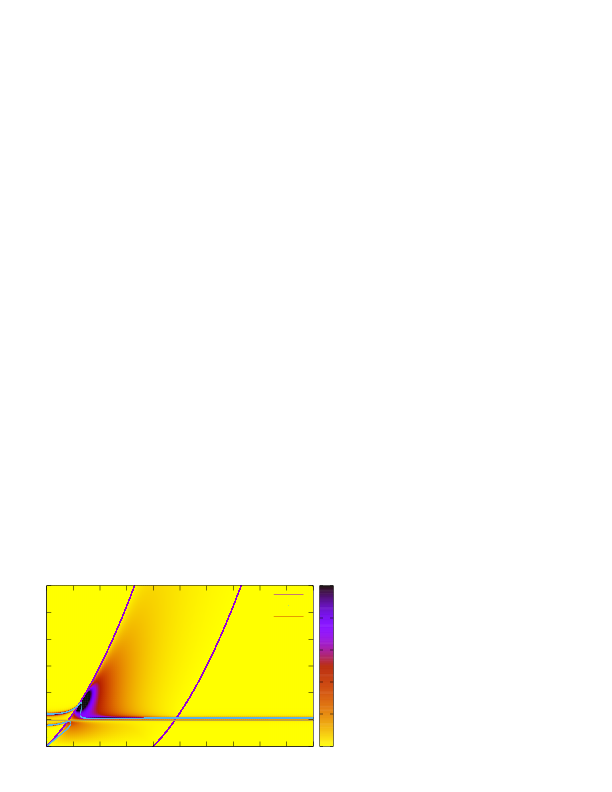
\includegraphics{plots/iminvepsGaAsn5e17Lindhard-damping}}%
    \gplfronttext
  \end{picture}%
\endgroup
